\chapter{Research Method}


%===================================================================================================%
\section{Introduction}
%===================================================================================================%


%===================================================================================================%
\section{Method Evaluation}
%=======================================================%

TTF vs ReqEng+FVM ?

"Characteristics" für Streaming und beide techs feststellen


%===================================================================================================%
\section{Prototyping}
%=======================================================%

managed container: IBM IoTP\\
serverless: AWS Kinesis+Firehose+Lambda

%***************%
\section{Requirement Engineering and Operationalization}\label{sec:operationalization}
%***************%

%***************%
\subsection{Viability Assessment}
%***************%

wie einfach war das deployment, blah

\begin{figure}[ht]
    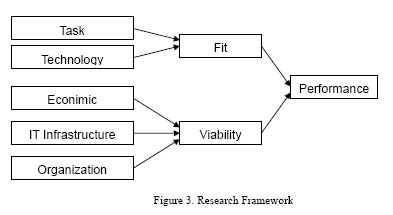
\includegraphics[width=0.7\linewidth]{images/methodology/fvm.jpg}\centering
    \caption
    [Fit-Viability-Model]
    {Fit-Viability-Model \cite{Liang2007AdoptionModel}}
\end{figure}

%***************%
\subsection{Suitability Assessment}
%***************%

\begin{enumerate}
    \item scaleabilitty
    \item microbilling
    \item loosely coupled
    \item event-driven
\end{enumerate}


\begin{figure}[ht]
    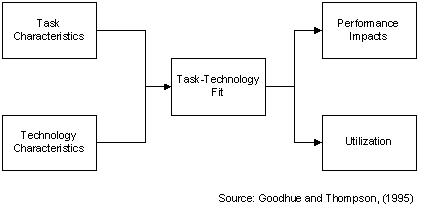
\includegraphics[width=0.7\linewidth]{images/methodology/ttf.jpg}\centering
    \caption
    [Task-Technology-Fit Model]
    {Task-Technology-Fit Model \cite{Goodhue1995Task-TechnologyPerformance}}
\end{figure}


%===================================================================================================%
\section{Summary}
%===================================================================================================%